\documentclass{article}

\usepackage{multicol}
\usepackage[utf8]{inputenc}
\usepackage[T1]{fontenc}
\usepackage{geometry}
\usepackage{minted}
\usepackage{xcolor}
\usepackage{hyperref}
\usepackage{framed}
\usepackage{amsmath}
\usepackage{float}
\usepackage{graphicx}
\usepackage{booktabs}

\title{Big Data For Engineers}
\author{Philip J. Hartout, Gian S. Hiltbrunner}
\date{June 2020}

\usepackage[sfdefault]{FiraSans}

\newminted[xml]{xml}{
    fontfamily = tt,
    fontsize = \normalsize,
    gobble = 1,
    samepage
}

\newminted[json]{json}{
    fontfamily = tt,
    fontsize = \normalsize,
    gobble = 1,
    samepage
}


\begin{document}
% \begin{multicols}{2}

\maketitle

\begin{center}
    \color{red}
    \begin{framed}
    \noindent Parts of the information provided within this document may be incomplete and/or incorrect. For corrections please submit a pull request to:
    \url{https://github.com/gianhiltbrunner/BigDataForEngineersSummary}
    \end{framed}
\end{center}

\tableofcontents

\section{Introduction}
\subsection{Are you capable of sketching the history of databases (ancient and modern) to a colleague in a few minutes?}

Early forms of databases include natural forms of information storage such as speaking, singing and writing. These forms became more complex in time when people performed simple accounting tasks using stone inscriptions and later on when books became widespread with the invention of the book press. The computer then finally enabled us to store and manage data on much larger scales.

In the 1960s file systems were introduced allowing simple forms of data managment, in the 1970s relational table databases such as SQL were introduced allowing systematic queries. In the 2000s other databases became more popular (NoSQL), these include key-value stores, triple stores, document stores and column stores.

\subsection{Do you know who Edgar Codd is?}

Edgar Codd was an English computer scientist who invented the relational model for database management, the theoretical basis for relational databases.

\subsection{Can you explain what Data Independence is, and why it is important?}

The actual data and application programs acting on the data remain unimpaired even if the storage representation or access methods are changed. This is important when we want to store small scale data on a single hard drive and store large scale data on cluster infrastructure but essentially want to access the data in the same manner.

\subsection{Do you know the rough conceptual difference between data, information, and knowledge?}

\begin{itemize}
    \item Data is conceived of as symbols or signs, representing stimuli or signals lacing any interpretation.
    \item Information is inferred from data", in the process of answering interrogative questions (e.g., "who", "what", "where", "how many", "when"), thereby making the data useful for "decisions and/or action".
    \item Knowledge represents information combined with understanding, capability and experience.
\end{itemize}


\subsection{Can you cite the five fundamental shapes of data, and how structured data can be characterized?}

Text, Tables, Trees, Graphs and Cubes

\begin{itemize}
    \item Data conforms to a data model and has easily identifiable structure
    \item Data is well organised so, Definition, Format and Meaning of data is explicitly known
    \item Data resides in fixed fields within a record or file
    \item Similar entities are grouped together to form relations or classes
    \item Entities in the same group have same attributes
    \item Easy to access and query, So data can be easily used by other programs
    \item Data elements are addressable, so efficient to analyse and process
\end{itemize}

\subsection{Can you briefly explain what a data model is?}

Underlying Questions

\begin{itemize}
    \item How does the data look like?
    \item What can be done with the data?
\end{itemize}

\noindent A data model is an abstract model that organizes elements of data and standardizes how they relate to one another and to the properties of real-world entities. For instance, a data model may specify that the data element representing a car be composed of a number of other elements which, in turn, represent the color and size of the car and define its owner.

\subsection{Do you know the 8 standard prefixes of the International System of Units (when the exponent in base 10 is a positive multiple of 3)?}

\begin{table}[H]
\begin{tabular}{|l|l|}
\hline
\textbf{Prefix} & \textbf{Digits} \\ \hline
kilo (k) & 1,000 (3 zeros) \\ \hline
Mega (M) & 1,000,000 (6 zeros) \\ \hline
Giga (G) & 1,000,000,000 (9 zeros) \\ \hline
Tera (T) & 1,000,000,000,000 (12 zeros) \\ \hline
Peta (P) & 1,000,000,000,000,000 (15 zeros) \\ \hline
Exa (E) & 1,000,000,000,000,000,000 (18 zeros) \\ \hline
Zetta (Z) & 1,000,000,000,000,000,000,000 (21 zeros) \\ \hline
Yotta (Y) & 1,000,000,000,000,000,000,000,000 (24 zeros) \\ \hline
\end{tabular}
\end{table}

\subsection{Can you list the main four technologies commonly referred to as NoSQL?}

\begin{itemize}
    \item Key-value stores
    \item Triple stores
    \item Column stores
    \item Document stores
\end{itemize}

\subsection{Do you know the three Vs?}


Big Data is defined by the three Vs.
\begin{itemize}
    \item \textbf{Volume}: High amount of data.
    \item \textbf{Variety}: Different types and structures.
    \item \textbf{Velocity}: High rate of data throughput.
\end{itemize}



\subsection{Can you briefly define capacity, throughput and latency? Do you know their typical units?}

\begin{itemize}
    \item \textbf{Capacity}: Volume of the stored data. (GB)
    \item \textbf{Throughput}: Speed of data transmission. (kbit/sec)
    \item \textbf{Latency}: Time until data is being received. (sec)
\end{itemize}

\subsection{Can you explain why and how the evolution of capacity, throughput and latency over the last few decades has influenced the design of modern databases?}

While the capacity has increased 200,000,000,000 fold, the throughput has increased only 10,000 fold and the latency only 8 fold.

\subsection{Can you name a few big players in the industry that accumulate and analyze massive amounts of data?}

Google, AWS (Amazon Web Services), Microsoft Azure and many more

\subsection{Do you know the difference between bit and byte?}

One byte is a collection of 8 bits where a bit represents the most basic form of information storage: 1 or 0.

\subsection{Can you name a few concrete examples that illustrate the various orders of magnitude of amounts of data?}



\pagebreak

\section{Lessons learnt}
\subsection{Can you explain why it is important to take into consideration whether a use case is read-intensive, or write-intensive, or in-between?}


Write Intensive $\rightarrow$ \textbf{OLTP} (On-line Transaction Processing) is involved in the operation of a particular system. OLTP is characterized by a large number of short on-line transactions (INSERT, UPDATE, DELETE). The main emphasis for OLTP systems is put on very fast query processing, maintaining data integrity in multi-access environments and an effectiveness measured by number of transactions per second. In OLTP database there is detailed and current data, and schema used to store transactional databases is the entity model (usually 3NF). It involves queries accessing individual record like updating an email record in a database.\\\\

\noindent Read Intensive $\rightarrow$ \textbf{OLAP} (On-line Analytical Processing) deals with historical data or archival data. OLAP is characterized by a relatively low volume of transactions. Queries are often very complex and involve aggregations. For OLAP systems a response time is an effectiveness measure. OLAP applications are widely used for data mining applications. In an OLAP database there is aggregated, historical data, stored in multi-dimensional schemas. Queries often access large amounts of data.

\subsection{Can you explain why normal forms are important?}

Normal forms are important to reduce data redundancy and improve data integrity. This is achieved by making sure that the data follows a set of rules corresponding to each of the normal forms.

\subsection{Can you describe the first normal form in simple terms?}

The first normal form expects the data to have a primary key ("id"), no repeating groups of entries (Not having columns such as "ChildName1" and "ChildName2") and atomicity of entries (No column such as "Children" with value e.g. "Max, Pia").

\subsection{Can you describe in simple terms (that is, without knowing the details of them) how higher normal forms (like Boyce-Codd) are related to joins?}

Higher order forms make sure that the data conforms to certain rules, thus when joining tables less conflicts occur.


\subsection{Can you explain why it is common, for large amounts of data, to drop several levels of normal form, and denormalize data instead?}

Denormalization is used to increase performance and scalability for large datasets. This leads to a increase in read performance while write performance suffers. This is due to the fact that relational databases need to perform many expensive JOIN operations when data is retrieved. These operations are prohibitively costly for very large datasets.

\begin{itemize}
    \item[+] Retrieving data is faster since we do fewer joins
    \item[+]Queries to retrieve can be simpler(and therefore less likely to have bugs), since we need to look at fewer tables.
    \item[-]Updates and inserts are more expensive.
    \item[-]Denormalization can make update and insert operations more complex.
    \item[-]Data may be inconsistent.
    \item[-]Data redundancy necessitates more storage.
\end{itemize}




\subsection{Can you give simple examples of denormalized data?}

\begin{figure}[H]
    \centering
    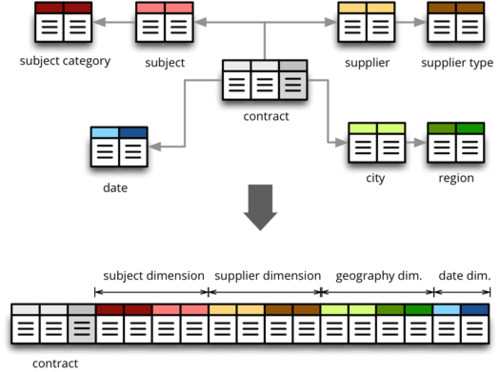
\includegraphics[width=0.3\linewidth]{img/denormalization.png}
\end{figure}

\subsection{Can you explain what a declarative language is?}

Declarative languages such as SQL describe what needs to happen but do not care about how exactly something is happening. Thus we would tell the the interpreter to fetch an entry using SELECT but not really care about how this entry is selected. (e.g. looping over the entries, etc.)

\subsection{Can you explain what a functional language is?}

Functional programming is a programming paradigm where programs are constructed by applying and composing functions. It is a declarative programming paradigm in which function definitions are trees of expressions that each return a value.

\subsection{Can you explain why it matters to design query languages that are declarative and functional?}

Declarative languages make sure that the we don't "reinvent the wheel" every time we create a query. Functional languages basically have similar benefits. They use functions to perform many operations such as map instead of looping over an array manually, thereby hiding away complexity and making code more readable.

\subsection{Can you describe the major relational algebra operators: select, project, group and aggregate, join, Cartesian product, union, intersection, etc?}

\begin{itemize}
    \item \textbf{SELECT}: Operation that subsets the data set given a condition. Such as SELECT all entries from the table Person whose age is larger than 34. ($\sigma_{\text{Age}\geq34}(\text{Person})$)
    \item \textbf{PROJECT}: Operation that picks a subset of all columns and drops duplicate entries. From table Person (Name, Age, Weight) project the columns Age and Weight to a new table while removing the Name column and excluding duplicate entries. ($ {\displaystyle \Pi _{\text{Age,Weight}}({\text{Person}})}$)
    \item \textbf{GROUP}: Operation that groups rows sharing the grouping property such that the groups can be aggregated in a subsequent operation. (e.g. SUM)
    \item \textbf{AGGREGATE}: Operation that summarizes multiple rows in a summarized form. Aggregate functions include: average, sum, median, standard deviation and many others.
    \item \textbf{JOIN}: Operation that unites two tables by the set of tuples that match. (e.g. key) \item \textbf{CARTESIAN PRODUCT}: Operation that creates a new table based on all possible combinations.
    \item \textbf{UNION}: Operation that combines tables from two SELECT operations.
    \item \textbf{INTERSECTION}: Operation that combines rows from tables that are present in both original data sets.
\end{itemize}

\subsection{Do you know what each letter stands for in ACID and CAP?}

\textbf{ACID}

\begin{itemize}
    \item Atomicity: Atomicity guarantees that each transaction is treated as a single "unit", which either succeeds completely, or fails completely.
    \item Consistency: Consistency ensures that a transaction can only bring the database from one valid state to another, maintaining database invariants.
    \item Isolation: Transactions are often executed concurrently (e.g., multiple transactions reading and writing to a table at the same time). Isolation ensures that concurrent execution of transactions leaves the database in the same state that would have been obtained if the transactions were executed sequentially.
    \item Durability: Durability guarantees that once a transaction has been committed, it will remain committed even in the case of a system failure (e.g., power outage or crash).
\end{itemize}

\noindent\textbf{CAP}

\begin{itemize}
    \item Consistency: Every copy of a data set has to be modified upon completion of a transaction. Note that this is not the same as consistency in the ACID model.
    \item Availability: Every request receives a (non-error) response, without the guarantee that it contains the most recent write
    \item Partition tolerance: The system continues to operate despite an arbitrary number of messages being dropped (or delayed) by the network between nodes
\end{itemize}

\subsection{Can you explain why, for large amounts of data, CAP becomes relevant over ACID?}

\noindent\textbf{ACID} addresses an individual node's data consistency\\
\textbf{CAP} addresses cluster-wide data consistency

\subsection{Do you know the names of the basic components of the tabular shape at an abstract level (table, row, column, primary key) as well as the names of the most common corresponding counterparts in the NoSQL world?}

\begin{table}[H]
\begin{tabular}{|l|l|}
\hline
\textbf{SQL} & \textbf{NoSQL} \\ \hline
database & database \\ \hline
table & collection \\ \hline
row & document \\ \hline
column & field \\ \hline
index & index \\ \hline
primary key & primary key \\ \hline
\end{tabular}
\end{table}

\subsection{Do you know the basic SQL constructs: SELECT FROM WHERE, GROUP, HAVING, JOIN, ORDER BY, LIMIT, OFFSET, as well as nested queries?}

\href{https://www.codecademy.com/articles/sql-commands}{Codecademy - SQL Commands}

\pagebreak

\section{Object storage}
\subsection{Can you describe the limitations of traditional (local) file systems?}

Local file systems are limited in capacity by the hardware capacity, i.e. they cannot contain petabytes. Local filesystems can also have local hierarchical and does not allow flexible manipulation of it.

\subsection{Can you explain what object storage is?}

Object storage (also known as object-based storage) is a computer data storage architecture that manages data as objects, as opposed to other storage architectures like file systems which manages data as a file hierarchy, and block storage which manages data as blocks within sectors and tracks. (Wikipedia)

It uses a flat, simple and global key value model and flexible metadata to enable retention of a massive amount of unstructured data.

\subsection{Can you explain what the benefits of object storage are?}

It enables the retention of massive, and diverse amounts of data on commodity hardware, with easy key-value pair access, and flexible metadata. Scaling out in terms of hardware with this approach allows also to have more performance for a lower price.

\subsection{Can you contrast or relate object storage with block storage, a file system, and the key-value model?}

See wiki entry again: object storage (also known as object-based storage) is a computer data storage architecture that manages data as objects, as opposed to other storage architectures like file systems which manages data as a file hierarchy, and block storage which manages data as blocks within sectors and tracks. (Wikipedia)

\subsection{What is the CAP theorem?}

In theoretical computer science, the CAP theorem, also named Brewer's theorem after computer scientist Eric Brewer, states that it is impossible for a distributed data store to simultaneously provide more than two out of the following three guarantees:

\begin{itemize}
\item Consistency: Every read receives the most recent write or an error
\item Availability: Every request receives a (non-error) response, without the guarantee that it contains the most recent write
\item Partition tolerance: The system continues to operate despite an arbitrary number of messages being dropped (or delayed) by the network between nodes
\end{itemize}

When a network partition failure happens should we decide to

\begin{itemize}
\item Cancel the operation and thus decrease the availability but ensure consistency
\item Proceed with the operation and thus provide availability but risk inconsistency
\end{itemize}

The CAP theorem implies that in the presence of a network partition, one has to choose between consistency and availability. Note that consistency as defined in the CAP theorem is quite different from the consistency guaranteed in ACID database transactions.

\subsection{Can you explain the three different ways, on the physical level, to deal with more data (scale up, scale out, write better code)?}

\begin{itemize}
\item Scale up - get bigger machines, price increases exponentially
\item Scale out - get more commodity machines, price increases linearly
\item Write better code - avoids excessive processing overhead and storage requirements, price can be substantially lower.
\end{itemize}

\subsection{Can you explain why scaling out is less expensive than scaling up?}

Because commodity hardware manufacturing is streamlined its price increases linearly, whereas harder to make and hence more expensive machines which are obtained by scaling up increase the cost exponentially.

\subsection{Can you explain what aspects of the design of object storage enable scaling out and why?}

The architecture is simple and can easily be fragmented to be stored on commodity hardware.

\subsection{Do you know what a data centre is made of (racks, server nodes, storage nodes, etc.)?}

Racks: vertical stack of server nodes. Storage nodes are server nodes or VMs specialized for storage.

\subsection{Do you know the difference between storage, memory, CPU and network and how the three are paramount in a cluster?}

Yes.

\subsection{Do you know rough, typical numbers (per-node storage capacity, memory, number of cores, etc.)?}

Typical data center: 1,000-100,000 machines
Cores: 1-100 cores per machine
Storage: 1-20 TB local storage per server
RAM: 16-6TB.
Network bandwidth:1-100 Gb/s

\subsection{Do you know how storage and memory technologies (HDD, SDD and RAM) compare in terms of capacity and throughput?}

Capacity HDD>SDD>RAM
Throughput HDD<SDD<RAM

\subsection{Can you sketch the (key-value) data model behind object storage? Can you spot instances of the key-value model in several other technologies seen in the lecture?}

\begin{figure}[H]
  \centering
  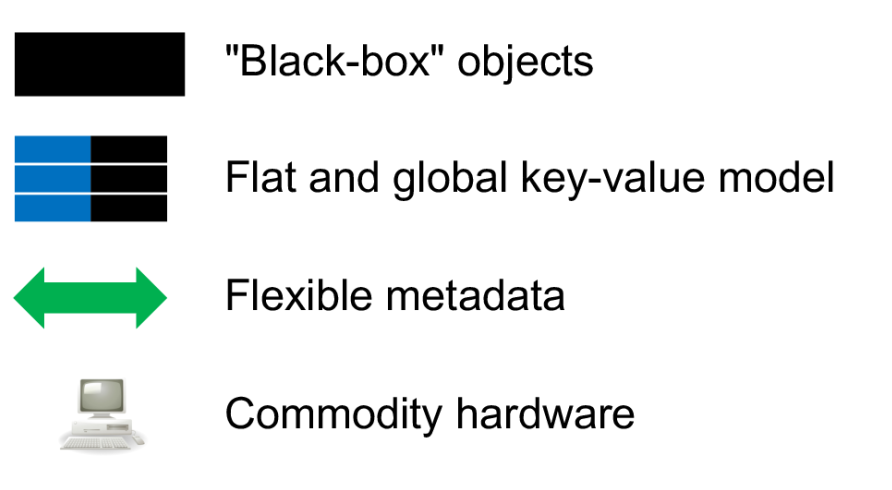
\includegraphics[width=.5\textwidth]{img/key_value_object_storage.png}
  \caption{Key value schema and other features of object storage}
  \label{fig:keyvalueobjectstorage}
\end{figure}

Other instances: JSON, Azure cosmos DB key value paradigm, ...

\pagebreak

\subsection{Do you know the difference between data and metadata?}

Metadata is data that provides information about other data. In other words, it is data about data.

\subsection{Do you know the order of magnitude that can be achieved in terms of number of objects, and object size?}

Object size ~5TB, 100 buckets per user by default.

\subsection{Can you name a few big players for cloud-based object storage (vendors, consumers)?}

Google, Microsoft, Amazon.

\subsection{Can you describe the features of S3 and Azure Blob Storage on a high level? Do you know what a bucket and object are? What block blob storage, append blob storage and page blob storage are and how they work?}

\begin{table}
  \centering
  \begin{tabular}{lll}
    \toprule
    & S3 & Azure \\
    \midrule
    Object ID & Bucket + Object & Account + container + blob \\
    Object API & Blackbox & Block Append Page \\
    Limit & 5TB & 4.78TB (block), 195TB (append), 8TB (page)\\
    \bottomrule
  \end{tabular}
  \caption{Overall comparison Azure vs S3}
  \label{tab:azurevss3}
\end{table}


\subsection{Can you describe what the most important SLA (Service Level Agreement) parameters mean (e.g., latency, availability, durability) as well as their typical range?}

\begin{table}
  \centering
  \begin{tabular}{ll}
    \toprule
    SLA & Outage \\
    99\% & 4 days/year\\
    99.9\% & 9 hours/year\\
    99.99\% & 53 minutes/year\\
    99.999\% & 6 minutes/year\\
    99.9999\% & 32 seconds/year\\
    99.99999\% & 4 seconds/year\\
    \bottomrule
  \end{tabular}
  \label{tab:sla}
  \caption{SLA}
\end{table}

Durability is loss of 1 in $10^{11}$ objects a year.

Response time is <10ms in $99.9\%$.

\subsection{Can you describe a typical use case for object storage?}


\begin{itemize}
\item Disaster recovery — Backup and Archiving.
\item Static web site hosting and static content distribution.
\item Document Store and file sharing.
\item Big Data analytics.
\end{itemize}

\subsection{Can you explain what a REST API is, what resources and methods are?}


Representational state transfer (REST) is a software architectural style that defines a set of constraints to be used for creating Web services. Web services that conform to the REST architectural style, called RESTful Web services, provide interoperability between computer systems on the Internet. RESTful Web services allow the requesting systems to access and manipulate textual representations of Web resources by using a uniform and predefined set of stateless operations. Other kinds of Web services, such as SOAP Web services, expose their own arbitrary sets of operations.

REST APIs use Uniform Resource Identifiers (URIs) to address resources. REST API designers should create URIs that convey a REST API's resource model to its potential client developers. When resources are named well, an API is intuitive and easy to use.

Methods include:
\begin{itemize}
\item HTTP GET
\item HTTP POST
\item HTTP PUT
\item HTTP DELETE
\item HTTP PATCH
\end{itemize}

Difference between PUT and PATCH: HTTP PATCH requests are to make partial update on a resource. If you see PUT requests also modify a resource entity, so to make more clear – PATCH method is the correct choice for partially updating an existing resource, and PUT should only be used if you’re replacing a resource in its entirety.

\subsection{Can you explain how an object storage API looks like (get and put)?}

You can address any combination of bucket and object name like so in S3:

\url{http://bucket.s3.amazonaws.com/object-name}

\subsection{Are you able to upload and download objects from S3 or Azure Blob Storage?}

Yes. This is also what one does when hosting a static website.

\pagebreak

\section{Distributed file systems}
\subsection{Can you explain the difference between block storage and object storage?}

\textbf{Block storage} is organised as blocks, which emulate the type of behaviour seen in traditional disk or tape storage. Blocks are identified by an arbitrary and assigned identifier by which they may be stored and retrieved, but this has no obvious meaning in terms of files or documents. A filesystem must be applied on top of the block-level storage to map 'files' onto a sequence of blocks. (Replication or backups)\\
\textbf{Object store} or 'bucket store', such as Amazon S3 (Simple Storage Service) operate at a higher level of abstraction and are able to work with entities such as files, documents, images, videos or database records. Each object typically includes the data itself, a variable amount of metadata, and a globally unique identifier.

\subsection{Can you explain the difference between the (logical) key-value model and a file system?}

The key value model is typically built on top of an object storage system while a file system works on block storage. 

\subsection{Can you contrast block storage and object storage in terms of maximum number of objects/files?}

\begin{itemize}
    \item \textbf{Key-Value Model}: Object Storage: Billions of sub-terabyte files. (Many small)
    \item \textbf{File System}: Block Storage: Millions of sub-petabyte files. (Few big)
\end{itemize}

\subsection{Can you contrast block storage and object storage in terms of the maximum size of objects/files?}

\begin{itemize}
    \item \textbf{Key-Value Model}: A terabyte
    \item \textbf{File System}: A petabyte
\end{itemize}

\subsection{Do you know the order of magnitude of a block size for a local file system and for a distributed file system? Can you explain the rationale behind them with respect to latency and throughput?}

\begin{itemize}
    \item \textbf{Local filesystem}: 4 kB
    \item \textbf{Distributed file system}: 64 MB - 128 MB
\end{itemize}

On a local system we have very high trougput and low latency, but on a cluster system the machines are connected over a network infrastructure which slows down transfer speeds. In order to make transfers more efficient larger blocks are used. 

\subsection{Do you know where HDFS shines and why?}

\begin{itemize}
    \item Works with varied data such as text, XML, CSV and many more. 
    \item Works on commodity hardware - Cheap
    \item High performance due to parallelization
    \item Fault-tolerant
    \item Scalable
\end{itemize}

\subsection{Do you know that HDFS files are updated by appending atomically and why?}

HDFS will always append to the last block and only one singe write operation is allowed at one time. Thus guaranteeing that there are no issues with concurrency.

\subsection{Do you know how HDFS performs in terms of throughput and latency?}

{\color{red} HDFS is optimized to access batches of data set quicker (high throughput), rather then particular records in that data set (low latency).}

\subsection{Do you know the main benefits of HDFS (commodity hardware, etc.)?}

See "Do you know where HDFS shines and why?".

\subsection{Can you contrast master-slave architectures to peer-to-peer architectures?}

n the master-slave model, one node is in charge (master). When there’s no single node with a special role in taking charge, you have a peer-to-peer distribution model.

\subsection{Can you explain the HDFS architecture, what a namenode is and what a datanode is, how blocks are replicated?}

HDFS works in a master-slave configuration. There is a master called the "Namenode" and multiple slaves called "Datanodes".

\begin{itemize}
    \item \textbf{Namenode}: Manages the file namespace, acess control file to block mapping and keeps track of the block locations. 
    \item \textbf{Datanode}: System that stores blocks on the local disk. 
    \item \textbf{Replication}: Blocks are replicated on multiple Datanodes for fault tolerance. 
\end{itemize}

\subsection{Can you sketch how the various components communicate with each other (client, namenode, datanode)?}

\begin{figure}
    \centering
    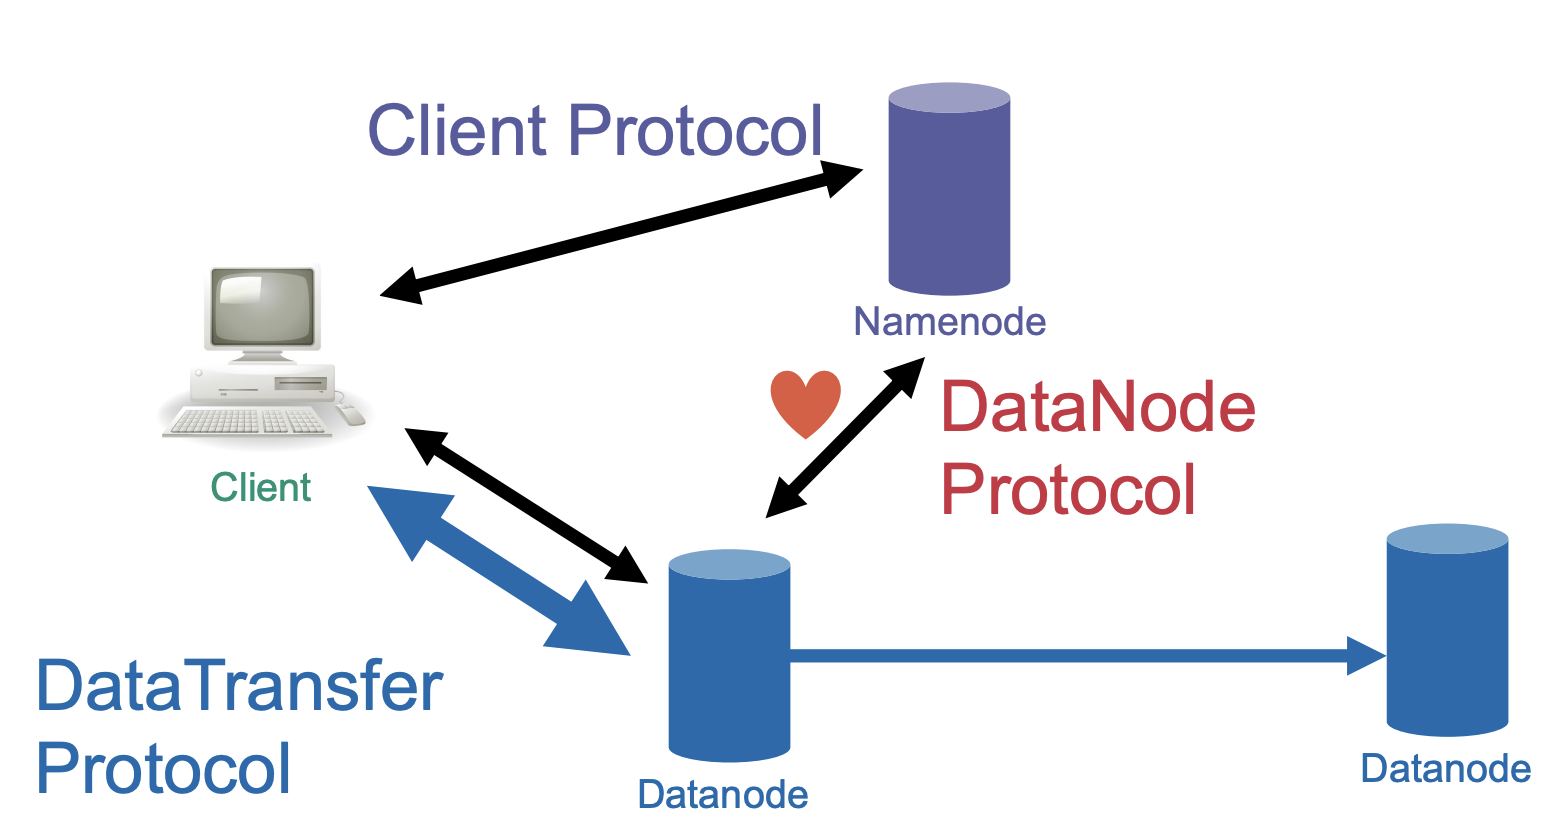
\includegraphics[width=0.5\linewidth]{img/hdfsoverview.png}
\end{figure}

\begin{itemize}
    \item \textbf{Client Protocol}: Manages metadata operations, DataNode locations and block IDs. 
    \item \textbf{DataNode Protocol}: Block operations such as replication managment and registration of the data node, heartbeat pings, block reports and block recieved confirmations. The DataNode always initiates the connection. 
    \item \textbf{Data Transfer Protocol}: Data blocks are transferred from a DataNode to a client or back. The datanode then initiates replication pipelining. 
\end{itemize}

{\color{red} Add precise data read and write protocol?}

\subsection{Can you point to the single points of failure of HDFS and explain how they can be addressed?}

The NameNode is a single point of failure. 

We resolve this using: 

\begin{itemize}
    \item \textbf{Persistance}: We store the inital namespace file and append an edit log with the changes that have been made. 
    \item \textbf{Backup}: We back this file up. 
\end{itemize}


\subsection{Can you explain how the namenode stores the file system namespace, in memory and on disk? In particular, can you explain how the namespace file and the edit log work together at startup time and how they get modified once the system is up and running?}
\subsection{Can you explain what a standby namenode is, what it is and what it is not?}
\subsection{Are you able to use the HDFS shell commands (creating directories, reading, uploading and downloading files, etc.)?}

\pagebreak

\section{Syntax}
\subsection{Can you describe why syntax is relevant to data management and to Big Data, for all data shapes?}

Syntax is crucial for efficient data management, and should be adapted to the data type is represents, e.g. if the data is in first normal form (i.e. there is atomic integrity) then csv is good, but if there is nestedness you will probably have data duplication, in this case JSON is more appropriate and avoids redundancy.

\subsection{What are the system demands for normalized vs. denormalized data?}

Normalized data is write intensive, e.g. if there is nestedness. Denormalized data is read intensive.

\subsection{What do normalized vs. denormalized data avoid?}

Normalized: avoid update anomalies
Denormalized: avoids joins.

\subsection{Can you give examples of syntax for trees? For tables? (The two data shapes extensively covered in the lecture)}

CSV for tables and JSON for trees.


\subsection{Can you explain what well-formedness is with respect to syntax?}

well-formedness in the case of JSON for instance is when all the rules of the JSON syntax are respected by a JSON string.

\subsection{Can you list the XML basic building blocks (we covered document, element, attribute, text) and do you know what they look like?}

They look like this:
\begin{center}
\begin{listing}[!ht]
  \begin{xml}
    <element attribute="value">
    Some text
    </element>
  \end{xml}
  \caption[Test]{XML building blocks}
  \label{lst:test}
\end{listing}
\end{center}


\subsection{Can you tell whether a given XML document is well-formed, with a software (oXygen) as well as with your own eyes?}

Well formed json string

\begin{center}
\begin{listing}[!ht]
  \begin{json}
    {
      "tissue_directories": [
            "gtex/brain/brain_cerebellar_hemisphere.tpm.csv"
      ],
      "tissue_names": [
            "Brain Cerebellar Hemisphere"
      ],
      "sample_strategy": [
            "mean",
            "mean"
      ],
      "expression_selection": [
            [
                  "smaller",
                  100
            ],
            [
                  "smaller",
                  100
            ]
      ]
    }
  \end{json}
  \caption[Test]{JSON well formed}
  \label{lst:test}
\end{listing}
\end{center}

\begin{center}
\begin{listing}[!ht]
  \begin{json}

      "tissue_directories": [
            "gtex/brain/brain_cerebellar_hemisphere.tpm.csv"
      ],
      "tissue_names" [
            "Brain Cerebellar Hemisphere"
      ],
      sample_strategy: [
            "mean"
            "mean"
      ],
      "expression_selection": [
            [
                  "smaller",
                  100
            ],
            [
                  smaller,
                  100
            ]
      ]

  \end{json}
  \caption[Test]{JSON not well formed}
  \label{lst:test2}
\end{listing}
\end{center}

Another example of not well-formed JSON.

\subsection{Do you know the five fundamental pre-defined entities (used to escape characters: $\&$ < > ' ") and their syntax?}

See Table~\ref{tab:predefinedentitites}.

\begin{table}
  \centering
  \begin{tabular}{lllll}
    \toprule
    Name & Character & Unicode code point (decimal) & Standard & Name\\
    \midrule
    quot & " & U+0022 (34) & XML 1.0 & quotation mark\\
    amp  & \& & U+0026 (38) & XML 1.0 & ampersand\\
    apos & ' & U+0027 (39) & XML 1.0 & apostrophe \\
    lt & < & U+003C (60) & XML 1.0 & less-than sign\\
    gt & > & U+003E (62) & XML 1.0 & greater-than sign\\
    \bottomrule
  \end{tabular}
  \caption{Predefined entities. }
  \label{tab:predefinedentitites}
\end{table}

\subsection{Do you know when some characters must be escaped (e.g., < in text)?}

Characters must be escaped in text. In JSON, done with ``\textbackslash". In XML, follow the conve
ntions shown in Table~\ref{tab:predefinedentitites}.

\subsection{Can you list the JSON basic building blocks (object, array, string, number, boolean,null) and do you know what they look like?}

Shown in Listing~\ref{lst:test}.

\subsection{Can you tell whether a given JSON document is well-formed, also with your own eyes?}

Try with Listings~\ref{lst:test} and ~\ref{lst:test2}.

\subsection{What is the difference between validation and well-formedness}

validation comes after well-formedness, i.e. a well formed string is validated against a schema, which is a well-formed JSON string. Example of a schema is shown in:

\begin{center}
 \begin{listing}
   \begin{json}
     {"type": "object",
    "properties": {
        "tissue_directories": {
            "type": "array",
            "items": {
                "type": "string"
            }
        },
        "tissue_names": {
            "type": "array",
            "items": {
                "type": "string"
            }
        },
        "sample_strategy": {
            "type": "array",
            "items": {
                "oneOf": [
                    {
                        "type": "string",
                        "enum": ["mean", "max", "min", "median"
                        ]
                    },
                    {
                        "type": "number", "minimum": 0, "maximum": 1
                    }
                ]
            }
        },
        "expression_selection": {
            "type": "array",
            "items": {
                "type": "array",
                "items": [
                    {
                        "oneOf": [
                            {
                                "type": "string",
                                "enum": ["greater", "smaller"
                                ]
                            },
                            {
                                "type": "number", "minimum": 0
                            }
                        ]
                    },
                    {
                        "type": "number","minimum": 0
                    }
                    ]
                  }
                }
              }
   \end{json}
    \caption[Test]{Example of schema (done to be compatible for \url{https://python-jsonschema.readthedocs.io/en/stable/})}
 \label{lst:test3}
 \end{listing}
\end{center}



\pagebreak

\section{Wide column stores}
\subsection{Can you explain the limitations of the traditional relational model?}
\subsection{Can you explain the differences and similarities between a wide column store and the traditional relational model?}
\subsection{Can you explain why wide column stores are called wide column stores, in particular on the storage level?}
\subsection{Do you know and can you contrast the two ways data can be distributed(partitioning, replicating)?}
\subsection{Can you explain the data model behind wide column stores, in particular, rows,columns, column families and cells?}
\subsection{Can you explain the motivation behind data getting denormalized into more columnfamilies?}
\subsection{Can you explain what aspects of an instance (table) in a column store must betypically known in advance, and which can be changed on the fly?}
\subsection{Can you name a few big players, in particular the one behind the initial founding paper?}
\subsection{Can you explain why HBase is based on HDFS, yet low-latency?}
\subsection{Can you explain what regions are for wide column stores?}
\subsection{Do you know how to identify a region based on the content of the wide column store?}
\subsection{Do you know the four basic kinds of (low-level) queries in HBase?}
\subsection{Can you describe the physical architecture of a wide column store like HBase, and compare it with that of a distributed file system like HDFS?}
\subsection{Do you know the physical layers of HBase (table, region, Store, Memstore, HFile,HBase block, Key Value)?}
\subsection{Do you know the difference between an HDFS block and an HBase block as well astheir typical sizes?}
\subsection{Can you explain how new cells are written to HBase via the cell store?}
\subsection{Can you explain how cells are read from HBase via both the stored HFiles and the Memstore?}
\subsection{Can you explain what compaction and flushing is?}
\subsection{Can you sketch the contents of an HFile and know what it corresponds to in anHBase table?}
\subsection{Can you explain why it is crucial not to have too long column family names?}
\subsection{Can you populate data into, and execute queries on top of HBase?}

\pagebreak

\section{Data models}
\subsection{Can you explain the difference between syntax and a data model?}
\subsection{Can you explain why and how trees can be used to model data that is denormalized(i.e., not in first normal form)?}
\subsection{Can you relate syntaxes to data models (e.g., CSV to tables, XML/JSON to trees, ...)?}
\subsection{Can you explain why trees modeling XML (infoset) have labels on the nodes, whiletrees modeling JSON have labels on edges?}
\subsection{Can you name a few data models for XML (Infoset, PSVI, XDM)?}
\subsection{Are you able, given an XML document, to sketch a tree representing that data (witha document node, elements, attributes, text, ...)?}
\subsection{Do you know the different between an atomic type/value, and a structuredtype/value (regardless of the exact data model)?}
\subsection{Can you name a few atomic types found across a broad number of data models?}
\subsection{Do you know the difference between the lexical space and the value space of anatomic type?}
\subsection{Can you tell the difference between structured types based on lists (e.g., JSON array) and maps (e.g., JSON object)?}
\subsection{Can you give examples of type cardinalities, and their associated symbols?}
\subsection{Can you explain the difference between well-formedness and validity? Do you knowwhat extra information you need to assess validity?}
\subsection{Are you able to design simple XML Schemas to validate XML? Can you restrict simpletypes to allow specific values or value fulfilling specific criteria (length, pattern...)? Can you explain how to declare elements with simple types? Can you explain how to declare elements with complex types and various content models (empty, simplecontent, complex content, mixed content)?}
\subsection{Can you tell, given an XML Schema, whether an XML document is valid against it,with software (oXygen) but also with your own eyes?}
\subsection{Are you able to design simple JSON Schemas to validate JSON?}
\subsection{Can you name (without details) further data modeling technologies for tree-likedata? (Avro, protocol buffers, ...)}
\subsection{Do you understand that a table in first normal form can be seen as a homogeneouscollection of flat trees (one per row and all with the same attributes)?}

\pagebreak

\section{Massive parallel processing (MapReduce)}
\subsection{Can you explain the patterns that appear in large-scale data processing: map, shuffle?}
\subsection{Can you explain how the mastery of these patterns can bring significant improvements in performance?}
\subsection{Can you explain the MapReduce model, also in terms of the patterns depicted above (map, shuffle, reduce)?}
\subsection{Can you describe the physical architecture of MapReduce (map tasks, reduce tasks as well as data flow)? Can you explain version 1 of the architecture (JobTracker, TaskTrackers) and its limits?}
\subsection{Can you outline what a map function looks like, and what a reduce function looks like?}
\subsection{Do you know the main input and output types of MapReduce?}
\subsection{Can you explain how combining improve MapReduce's performance?}
\subsection{Can you state the assumptions behind reusing the reduce function as a combinefunction?}
\subsection{Do you understand, in some simple cases, how to design a combine function thatwould make a MapReduce job faster, even if the combine function is not the exact same as the reduce function? (Example: computing an average, which requires keeping track of the weights in the output of the combine function).}
\subsection{Can you explain why MapReduce shines on top of a distributed file system: "Bring the query to the data"?}
\subsection{Can you explain why MapReduce especially makes sense when the bottleneck is the speed of reading and writing data from the disk (as opposed to other bottlenecks such as storage capacity or CPU usage)?}
\subsection{Can you explain how MapReduce splits differ from HDFS blocks, what impedance mismatches arise and how they are addressed?}
\subsection{Do you know what the Java API of MapReduce looks like on a high level (Version 2 of the API that we covered, not to be confused with Version 2 of MapReduce running on YARN)?}

\pagebreak

\section{Resource Management}
\subsection{Can you explain how YARN works, and how it can be used to improve MapReduce, and to support other technologies like Spark?}
\subsection{Can you describe the YARN components?}
\subsection{Do you know what a ResourceManager does?}
\subsection{Do you know what a NodeManager does?}
\subsection{Do you know what and where a Container is?}
\subsection{Do you know what an ApplicationMaster is and does?}
\subsection{Can you list the main resources that are managed in a cluster? (Disk storage,memory, CPU, network I/O).}
\subsection{Can you explain, in simpler words, what the added value of YARN is? Can you explainwhat it is an improvement over the first version of MapReduce, which was taking care of resource management on its own, and had issues with this?}

\pagebreak

\section{Massive parallel processing (Spark)}
\subsection{Can you explain how Spark is more powerful than MapReduce on a data model level?}
\subsection{Can you explain what a Resilient Distributed Dataset (RDD) is?}
\subsection{Do you know the difference between an action and a transformation?}
\subsection{Do you know the main actions and transformations available in Spark?}
\subsection{Are you able to classify transformations and actions in various buckets (those thatwork on any value, those that work on key-value pairs, unary binary transformations, ...)?}
\subsection{Can you describe how transformations run physically (tasks, stages...)?}
\subsection{Can you explain when and how a series of transformations can be optimized bykeeping the same set of machines with no network communication between the transformations?}
\subsection{Can you explain what a stage is? Can you relate it to transformations? To tasks? ToJobs?}
\subsection{Can you tell why and when shuffling is needed? In other words, can say whether atransformation has a narrow dependency or a wide dependency?}
\subsection{Can you easily draw a directly acyclic graph for a Spark job, and mark the stages?}
\subsection{Do you understand why keeping an RDD persisted can be useful and improveperformance?}
\subsection{Can you explain how controlling the way data is partitioned can make executionfaster because we can influence stages?}
\subsection{Can you explain what a DataFrame is and what its benefits are?}
\subsection{Can you describe the limitations of DataFrames?}
\subsection{Can you write queries on DataFrames, both in Spark SQL or using DataFramestransformations?}

\pagebreak

\section{Document stores}
\subsection{Do you understand how collections in documents store generalize the concept of a relational table?}
\subsection{Can you explain what documents store can do that relational databases cannot (e.g., heterogeneous collections, schema-less collections, data denormalized into trees...)?}
\subsection{Do you know how to issue MongoDB queries on a low level? Do you know the parameters of the find() function? (query, then projection, then sorting)?}
\subsection{Can you explain how, in a document store, the documents can be sharded and replicated?}
\subsection{Do you understand how indices can make queries faster, like in relational databases?}
\subsection{Do you know what kinds of indices there are (hash, B-trees)?}
\subsection{Are you capable of telling if an index is useful to a given query, for simple settings(for example, an index on a single field and a query that selects on that field)?}
\subsection{Do you know that a compound index (e.g., on keys a and b) can also be used as anindex on any prefix of the compound key (e.g., on key a only) "for free"?}

\pagebreak

\section{Querying trees}
\subsection{Can you explain why a language such as JSONiq provides, in the context of document stores, exactly the same functionality as SQL in a relational database?}
\subsection{Can you name the first-class citizen of the JDM (sequence of items)?}
\subsection{Can you name various kinds of items in the JDM?}
\subsection{Can you name a few query languages in the XML/JSON ecosystem?}
\subsection{Are you able, in JSONiq, to construct items (atomic items, elements, etc.)?}
\subsection{Are you able, in JSONiq, to perform logical operations? Do you understand what theEffective Boolean Value of a sequence and how it relates to logical operations?}
\subsection{Are you able, in JSONiq, to perform arithmetic operations (addition, etc.)? Do youunderstand the constraints on the input sequences of such operations? Can you explain the behavior of these operations on empty sequences? Can you explain what happens if one of the two operands is a node and not an atomic item?}
\subsection{Are you able, in JSONiq, to perform comparisons (lt, ge, etc.)? Do you understand the constraints on the input sequences of such operations? Can you explain the behavior of these operations on empty sequences? Can you explain what happens if one of the two operands is a node and not an atomic item?}
\subsection{Do you understand how general comparisons (<, >=, etc.) work on sequences with more than one item, and implicitly use an existential quantifier)?}
\subsection{Do you understand how FLWOR expressions work and describe what they return? (for clause, let clause, where clause, order by clause, etc.)}
\subsection{Are you able to use further expressions (if-then-else, switch, ...)?}
\subsection{Do you understand how to dynamically build JSON content with object and arrayconstructors?}
\subsection{Do you understand that expressions can be combined at will, as any expression takesand returns sequences of items? Do you know how to use parentheses to make precedence clear, like you did in primary school with + and *?}
\subsection{Do you know the JSONiq type syntax (atomic types taken from XML Schema, syntaxfor object and array types, as well as cardinality symbols), and how to use typechecking (instance of, cast as, etc.)?}
\subsection{Given a collection of JSON objects (for example JSON Lines on HDFS), are you able touse Rumble to write JSONiq queries (FLWOR) that do projection? selection? (weleave grouping, join, ... aside in the context of this lecture, however you need to know that this can be done with JSONiq as well).}

%\end{multicols}
\end{document}
% Local Variables:
% TeX-command-extra-options: "-shell-escape"
% End: